\documentclass{article}
\usepackage{graphicx} % Required for inserting images
\usepackage{amsmath} 
\usepackage{amssymb}
\usepackage{xcolor}
\usepackage[margin=1.2in]{geometry}

\title{this is an overleaf file}
\author{Patryk Drozd and Adriana Voloshyna }
\date{February 2024}

\begin{document}

\maketitle

\section{Background}
In extraordinary world of fluid mechanics, the Navier-Stokes equations remain the most reliable tool in understanding the motion of fluids. Developed over numerous decades by some of history's brightest minds, these equations are still used in modern day scientific research and have practical applications in engineering. In the 19th century, French engineer Claude-Louis Navier and  Irish physicist and mathematician Sir George Gabriel Stokes independently derived differential equations to describe the flow of a viscous fluid. Prior to this, the Euler equations provided the best description of fluid motion, but these equations did not account for the viscosity of a fluid. This oversimplification was a leading cause of deviation of experimental observations from theory. The Navier-Stokes Equations, although being a more accurate description of physical fluid behaviour, come with a mathematical cost. It has not been proven that these equations always have smooth (i.e. infinitely differentiable) solutions in three dimensions. This conundrum is of great interest to the mathematical community, and is one of the seven Millenium Prize Problems, meaning that the Clay Mathematics Institute has offered a prize of one million US dollars for the first correct proof of existence and smoothness or a counterexample. 

\section{Introduction}
Before we attempt to claim the one million dollar prize, we must first study a simpler case of the Navier-Stokes Equations. The aim of this paper is to investigate the use of computational methods to solve the equations in the two dimensional case. In particular, rather than solving the equations as a whole, our objective is to understand the individual terms in the equations in hopes of gaining a deeper insight into the fundamental structure of a fluid. Several computational methods were considered, such as the Finite Volume Method (FVM), Finite Difference Method (FDM), and the Finite Element Method (FEM).
\subsection{Computational Methods}
The Finite Volume Method involves subdividing a space (or volume) into a finite number of cells, creating a discretised collection of what are known as control volumes. Given a partial differential equation which can be written in divergence form, we can use Gauss' Divergence Theorem to rewrite a volume integral into a surface integral, and calculate the flux at each of the surfaces of the cells. This method relies on the conservation of flux, i.e. that the outward flux in each cell must be equal in magnitude to the inward flux entering the cell.

The Finite Difference Method is the most straightforward way to numerically solve a system of differential equations. The domain is discretised into a finite set nodal points, and the derivatives in question are approximated using finite difference (usually a central finite difference). This just means that we take the definition of a derivative from First Principles, but instead of finding the limit as the differential (the small change in x) goes to zero, we give it a very small but non-zero value. Then, for each nodal point we can find the value of a solution at that point, which together gives a numerical solution to a given system of differential equations. This method is efficient in computing solutions on a rectangular domain, but it is difficult to implement on an irregularly shaped domain.

The Finite Element Method also begins with discretising a domain into a finite number of elements. These elements are geometric shapes which together create a mesh for the given domain. To obtain a solution, a set of differential equations together with boundary conditions must first be expressed in what is known as the weak formulation. Then, for a given set of basis functions, we can find a solution for each element of the mesh and together this gives a solution to the system. This method is more mathematically involved than the others and has the least limitations on what type of equations or domains it can be used for. We thus decided that this method would not only be best suited to our problem, but also would be interesting to learn for its own sake.
\subsection{The Navier-Stokes Equation}
Observe below the Navier-Stokes Equation
$$\rho \frac{Du}{Dt} = - \nabla p + \mu \nabla^2u + F$$
where 
\begin{itemize}
\item $\rho$ is the fluid density 
\item {\Large$\frac{Du}{Dt} $} = {\Large$\frac{\partial u}{\partial t}$} $+\, u\nabla u$ is the acceleration of the fluid 
\item $p$ is the fluid pressure
\item $\mu$ is the fluid dynamic viscosity and 
\item $F$ is external force (often gravity).
\end{itemize}
This equation is derived from Newtons Second Law, where we have the sum of forces on one side of the equation, and density (instead of mass) multiplied by acceleration on the other side. We approach this equation by learning how to solve individual terms of the equation using FEM. For instance, to understand how to numerically compute the Laplacian term $\mu \nabla^2u$, we first aim to solve $\nabla^2u = f$, also known as the Poisson equation. Together with Dirichlet boundary conditions, we begin by understanding how to solve this equation in one dimension. Furthermore, we extend this notion to solving the Poisson problem in the two dimensional case, and develop an understanding of vector partial differential equations. We also wish to investigate the non-linearity of the equation, so we aim to solve a simpler problem, namely a non-linear Poisson equation. Similarly, to better our understanding of the time-dependent term, we intend to solve the two dimensional heat equation. This project will allow us to simultaneously study the Finite Element Method of solving various partial differential equations, and its relevance in searching for a solution to the Navier-Stokes equation. 

\section{Background of the Finite Element Method}
The Finite Element Method is a numerical method of solving differential equations. It can accurately approximate a solution to a boundary value problem when analytic solutions are difficult or impossible to find. Using this method we can model and study physical phenomena such as heat transfer, structural behaviour, fluid flow and electromagnetic potential. Finite Element Analysis is often used in engineering as it can accurately replicate simulations of different types of conditions in a cost effective, safe and efficient way. A very early example of this was NASTRAN, an open source Finite Element Analysis program developed for NASA in the 1960s to aid engineers in structural analysis. The program was so successful that it is still used in aerospace, maritime and automotive industries across the globe today. 

\section{One Dimensional Poisson Problem}
To gain an understanding of the algorithm behind the Finite Element Method, we begin by solving the one dimensional Poisson problem. Thus we want to find solutions \textit{u} which satisfy the differential equation

\[\nabla^{2}u = f  \qquad\textrm{on domain }\Omega \]
with the boundary condition 

\[u = 0 \qquad\textrm{on } \partial\Omega\]
Note that in the one dimensional case, the Laplacian $\nabla^{2}$ is simply the second derivative of u. Taking the domain to be the open interval (0,1), the differential equation reduces to 

$$ u'' = f \qquad\textrm{on }[0,1] $$
and the boundary condition can be written as
$$ u(0) = u(1) = 0. $$

The above is what is known as the strong formulation of the Poisson problem. We can express this alternatively using the weak formulation.
\subsection{Derivation of the Weak Formulation}
The weak formulation of the one dimensional Poisson problem can be described as follows:\\
\\
Given a function space 
$$ V := \{v| \textrm{ $v$ is continuous on [0,1], $v'$ is piecewise continuous and bounded on } [0,1],  v(0) = v(1) = 0 \} $$
we must find a $u$ $\epsilon$ $V$ such that 
\[(u',\phi ') = (f , \phi) \qquad\forall\,\phi\, \epsilon\, V\]
where 
$(u,v) := \int_{0}^{1} u(x)v(x) \,dx $
is the scalar product of functions u and v on [0,1].\\
\\
To see that these are equivalent, observe that if $-u'' = f$, we can multiply both sides by a test function $\phi$ and integrate over our domain to obtain 
\[-\int_{0}^{1} u"(x)\phi(x) \,dx = \int_{0}^{1} f(x)\phi(x) \,dx \qquad\forall\,\phi\, \epsilon\, V\]
after which we can use integration by parts to rewrite this as
\[- ( [u'(x)\phi(x)]_0^1 - \int_{0}^{1} u'(x)\phi'(x) \,dx ) = \]
\[\int_{0}^{1} u'(x)\phi'(x) \,dx - [ u'(1)\phi(1) - u'(0)\phi(0) ] = \int_{0}^{1} f(x)\phi(x) \,dx
\qquad\forall\,\phi\, \epsilon\, V. \]
But since $\phi$ $\epsilon$ $V$ , it must satisfy the boundary conditions $\phi(0)$ = $\phi(1)$ = 0, which causes the above to reduce to
\[\int_{0}^{1} u'(x)\phi'(x) \,dx  = \int_{0}^{1} f(x)\phi(x) \,dx \qquad\forall\,\phi\, \epsilon\, V \qquad\textrm{ as required.}\] 
\\
\\
To show implication in the other direction, and therefore proving equivalence, we repeat the steps above in the reverse direction. Let 
\[(u',\phi ') = (f , \phi) \qquad\forall\,\phi\, \epsilon\, V  \]
and take away 0 from the left side of the equation by using the boundary conditions which $\phi$ must satisfy
\[(u',\phi ') - [u'(1)\phi(1) - u'(0)\phi(0)] = (f , \phi) \qquad\forall\,\phi\, \epsilon\, V.  \]
We observe that the above can be reduced to 
\[(u'',\phi ) = (f , \phi) \]
which can be rewritten as 
\[(u'',\phi ) - (f , \phi) = (u'' - f,\phi )   = 0 \]
Since this must hold $\forall\,\phi\, \epsilon\, V$, we can conclude that
\[u'' - f = 0 \qquad \textrm{on }(0,1)\]
and so we have that the strong and weak form are equivalent. 
\subsection{Discretisation of the the Function Space}
Since computers of our age are not comfortable with infinities, we must discretise the infinite dimensional function space $V$, into a finite dimensional subspace $V_h$. To do so, we must create a mesh on which we will use basis functions to approximate a solution to our problem. This mesh provides a way of dividing our continuous domain, in this case the interval [0,1], into a finite amount of nodal points (or vertices) $x_i$ with 
$x_0 = 0$,..., $x_{n} = 1$.

On the interval between each nodal point $(x_i, x_{i+1})$, we can define a \textbf{Finite Element} $(K, P, \Sigma)$  where \\
- K is a cell of the mesh, also called an element \\
- P are polynomials on K and \\
- $\Sigma$ is a set of degrees of freedom. \\
Note that for this problem we will be working only with $\Sigma$ = 1, as our basis functions will be linear. If, for example, we wanted to use quadratic polynomials as our basis functions, we would set $\Sigma$ = 2, but for the purpose of solving the one dimensional Poisson problem, this would add an unnecessary degree of complexity. \\
\\
Now we have the tools to construct our finite dimensional subspace,
$$ V_h := \{v| \textrm{ $v$ is continuous on [0,1], } v|_{K_i}\, \epsilon\, P \textrm{ for each } i,\,  v(0) = v(1) = 0 \}. $$

\subsection{Basis Functions}
  The basis functions $\phi_i$ are simple polynomials which can be used to describe an element of our finite dimensional subspace $V_h$. A function $v$ has a unique representation in $V_h$ given by 
 $v_h(x) = \sum_{i=0}^{n}v_i\phi_i(x)$ where $n$ is the amount of nodal points in our interval, as before. Each basis function will be scaled by a constant $v_i$, and must satisfy $$\phi_i(x_j) =  \begin{cases} 
      1 & i = j \\
      0 & i \neq j.
   \end{cases}$$
Say for example we want to construct a function $v_h(x) = 1\cdot \phi_{0.25}(x) + 1\cdot \phi_{0.5}(x) + 1\cdot \phi_{0.75}(x)$. The figure below shows how the sum of the individual (scaled) bases superimpose to form our function. 
\begin{figure}[hbt!]
    \centering
    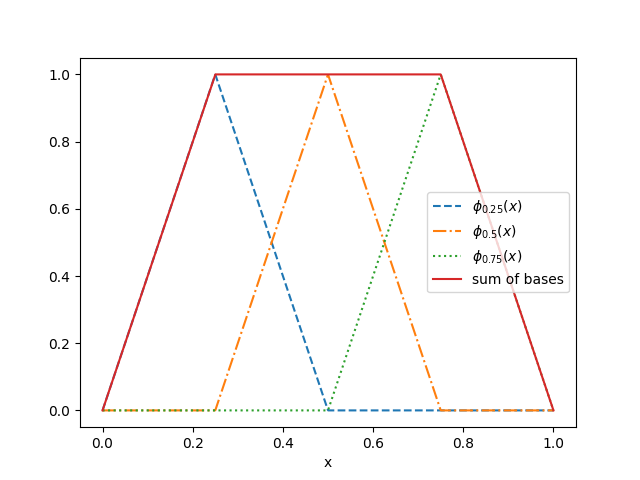
\includegraphics[width=10cm]{basis functions/linear_basis_sum.png}
    \caption{Sum of linear bases}
    \label{fig:linear basis sum}
\end{figure}
\subsection{Discretisation of the Weak Formulation}
The weak form of the Poisson problem can now be discretised to the following:
For a function space $V_h$ (as described previously), we must find a $u_h$ $\epsilon$ $V_h$ such that 
\[(u_h',\phi_h ') = (f , \phi_h) \qquad\forall\,\phi_h\, \epsilon\, V_h.\]
We can write $u_h'$ in terms of its basis functions to obtain:
\[((\sum_{j=0}^{n}u_j\phi_j'),\phi_h ') = (f , \phi_h) \qquad\forall\,\phi_h\, \epsilon\, V_h.\]
Furthermore, since any function $\phi_h$ can be written as a linear composition of basis functions, it is enough to show that
\[((\sum_{j=0}^{n}u_j\phi_j)',\phi_i ') = (f , \phi_i) \qquad\forall\,1 \leq i \leq n\]
\[\iff \sum_{j=0}^{n}u_j(\phi_j',\phi_i ') = (f , \phi_i) \qquad\forall\,1 \leq i \leq n. \]
Now we search for a sequence of constants $(u_j)$ which satisfy the equivalence above. 
\subsection{Linear System Representation}
To do this computationally, we can represent the linear system in the form of a matrix equation
\[\begin{pmatrix}
(\phi_1',\phi_1 ') & (\phi_1',\phi_2 ') & \hdots &(\phi_1',\phi_n ')\\
(\phi_2',\phi_1 ') & (\phi_2',\phi_2 ') & \hdots &(\phi_2',\phi_n ')\\
\vdots &  \vdots &  \ddots &  \vdots\\
(\phi_n',\phi_1 ') & (\phi_n',\phi_2 ') &\hdots &(\phi_n',\phi_n ')
\end{pmatrix}
\begin{pmatrix}
u_1\\
u_2\\
\vdots\\
u_n
\end{pmatrix} =
\begin{pmatrix}
(f , \phi_1) \\
(f , \phi_2) \\
\vdots\\
(f , \phi_n)
\end{pmatrix}\]
to find a vector $\vec{u}\ \epsilon\ \mathbb{R}^n$ which satisfies this equation. For clarity, let us rewrite the above equation as $$A \vec{u} = F$$ Solving a linear system like this is not difficult - we simply multiply both sides of the equation with the inverse of $A$ to obtain what $\vec{u}$ is equal to. All that remains is to find the components of $A$, i.e. the scalar product of the basis functions. 
\subsection{Matrix $A$}
Due to the symmetry of the matrix, we begin by solving the diagonal elements, which are all of the form $(\phi_i',\phi_i')$. In the figure below, we have one basis function $\phi_i$ which is non-zero only on the interval $[x_{i-1}$, $x_{i+1}]$. If h is the distance from $x_{i-1}$ to $x_{i}$ and the height of the basis function is set to 1, then $\phi_i(x) = x/h$ when restricted to the interval $[x_{i-1}$, $x_{i}]$. By symmetry, $\phi_i(x) = 1 - x/h$ on the interval $[x_{i}$, $x_{i+1}]$.  Then 
$$\int_{0}^{1} \phi_i'(x)\phi_i'(x) \,dx = \int_{x_{i-1}}^{x_{i+1}} \phi_i'(x)\phi_i'(x) \,dx = \int_{x_{i-1}}^{x_{i}} \left(\frac{1}{h}\right)\left(\frac{1}{h}\right)\,dx\, + \int_{x_{i}}^{x_{i+1}} \left(-\frac{1}{h}\right)\left(-\frac{1}{h}\right) \,dx $$ 
$$= \left[\frac{x}{h^2}\right]_{x_{i-1}}^{x_{i}} + \left[\frac{x}{h^2}\right]_{x_{i}}^{x_{i+1}} = \frac{h}{h^2} + \frac{h}{h^2} = \frac{2}{h}.$$ 
Now to find the elements next to the diagonal, we must calculate $(\phi_i',\phi_i+1')$ = $(\phi_i+1',\phi_i')$. Since $\phi_i = 0$ anywhere outside the interval $[x_{i-1}$, $x_{i+1}]$, we can limit our integral to the same interval. Moreover, $\phi_i+1 = 0$ on the interval $[x_{i-1}$, $x_{i}]$, so we can further restrict our limits of integration to $x_{i}$ and $x_{i+1}$. 
$$\int_{x_{i}}^{x_{i+1}} \phi_i'(x)\phi_{i+1}'(x) \,dx = \int_{x_{i}}^{x_{i+1}} \left(-\frac{1}{h}\right)\left(\frac{1}{h}\right)\,dx  = \left[-\frac{x}{h^2}\right]_{x_{i}}^{x_{i+1}} = -\frac{1}{h}.$$ 
Finally observe that any matrix elements other than those which we have calculated must equal to zero, as the two basis functions in the scalar product will never be non-zero on the same interval. This gives us a sparse matrix, one in which only a small number of entries are non-zero, which can save a lot of memory and storage space when searching for solutions to our linear system.  
\subsection{Matrix $F$}
To begin solving the left hand side of the equation, we must chose a function $f$. For the sake of simplicity, let $f = -1$. Then, for any basis function $\phi_i(x)$ which is not on the boundary of our domain, $$(f , \phi_i) = \int_{0}^{1} f(x)\phi_i(x) \,dx  = (- 1) \int_{x_{i-1}}^{x_{i+1}} \phi_i'(x) \,dx = - \int_{x_{i-1}}^{x_{i}} \left(\frac{x}{h}\right)\,dx\, - \int_{x_{i}}^{x_{i+1}} \left(1 -\frac{x}{h}\right) \,dx = - h.$$ 
Otherwise, $(f , \phi_1) = (f , \phi_n) = 0$, due to the boundary conditions $\phi_h$ must satisfy.
\subsection{Numerical Implementation and Solution}
Although it is possible to solve the scalar products of basis functions analytically, it can become tedious for large mesh sizes and non linear basis functions. Using the trapezoidal integration function (np.trapz), we can solve for the elements of the matrix numerically. To see that this numerical method can reproduce the same results that we achieved analytically, we plotted the elements of the matrix $A$. Observe in the figure above the results for a system with 9 nodal points and a system with 50 nodal points. Indeed we get a sparse matrix with non-zero elements only along the diagonal and one above or below the diagonal.
\begin{figure}[hbt!]
\centering
\begin{minipage}{.5\textwidth}
    \centering
    \includegraphics[width=8cm]{poisson 1d/(Poisson_1d)_(lin_matrix_A)_(x)_(vertex_num_9).png}
    \caption{Matrix A for 9 nodal points}
    \label{fig:Matrix A for 9 nodal points}

\end{minipage}%
\begin{minipage}{.5\textwidth}
    \centering
    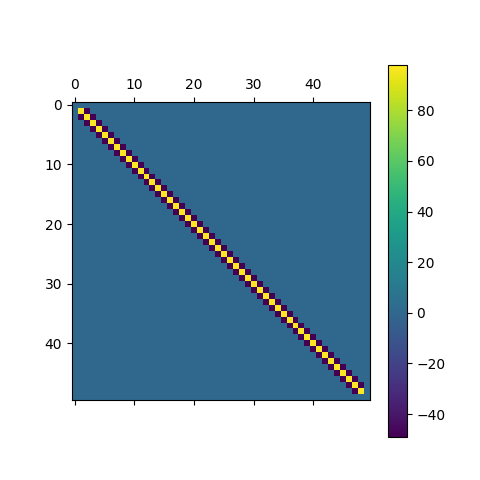
\includegraphics[width=8cm]{poisson 1d/(Poisson_1d)_(lin_matrix_A)_(x)_(vertex_num_50).png}
    \caption{Matrix A for 50 nodal points}
    \label{fig:Matrix A for 50 nodal points}

\end{minipage}
\end{figure}
\\
\\
Now that we have a linear system $A \vec{u} = F$, and the tools to obtain this equation numerically, we can look for solutions $\vec{u}$. To do this, it is necessary to create three nested for loops. For each element of our mesh, we find the scalar product of our function $f$ with our basis functions $\phi_i$ for all $i$. Then, for each basis function $\phi_i$, we take the scalar product of $\phi_i$ and $\phi_j$, for all $j$, which gives us a row of the matrix $A$ for each iteration of $i$. Using numpy.linalg.pinv we find the inverse of this matrix, and thus solve for $\vec{u}$. We are now ready to plot $\vec{u}$ to see the solutions to the one dimensional Poisson problem. Note how the curve is smoother when we consider a finer mesh with more nodal points. 
\begin{figure}[hbt!]
\centering
\begin{minipage}{.5\textwidth}
    \centering
    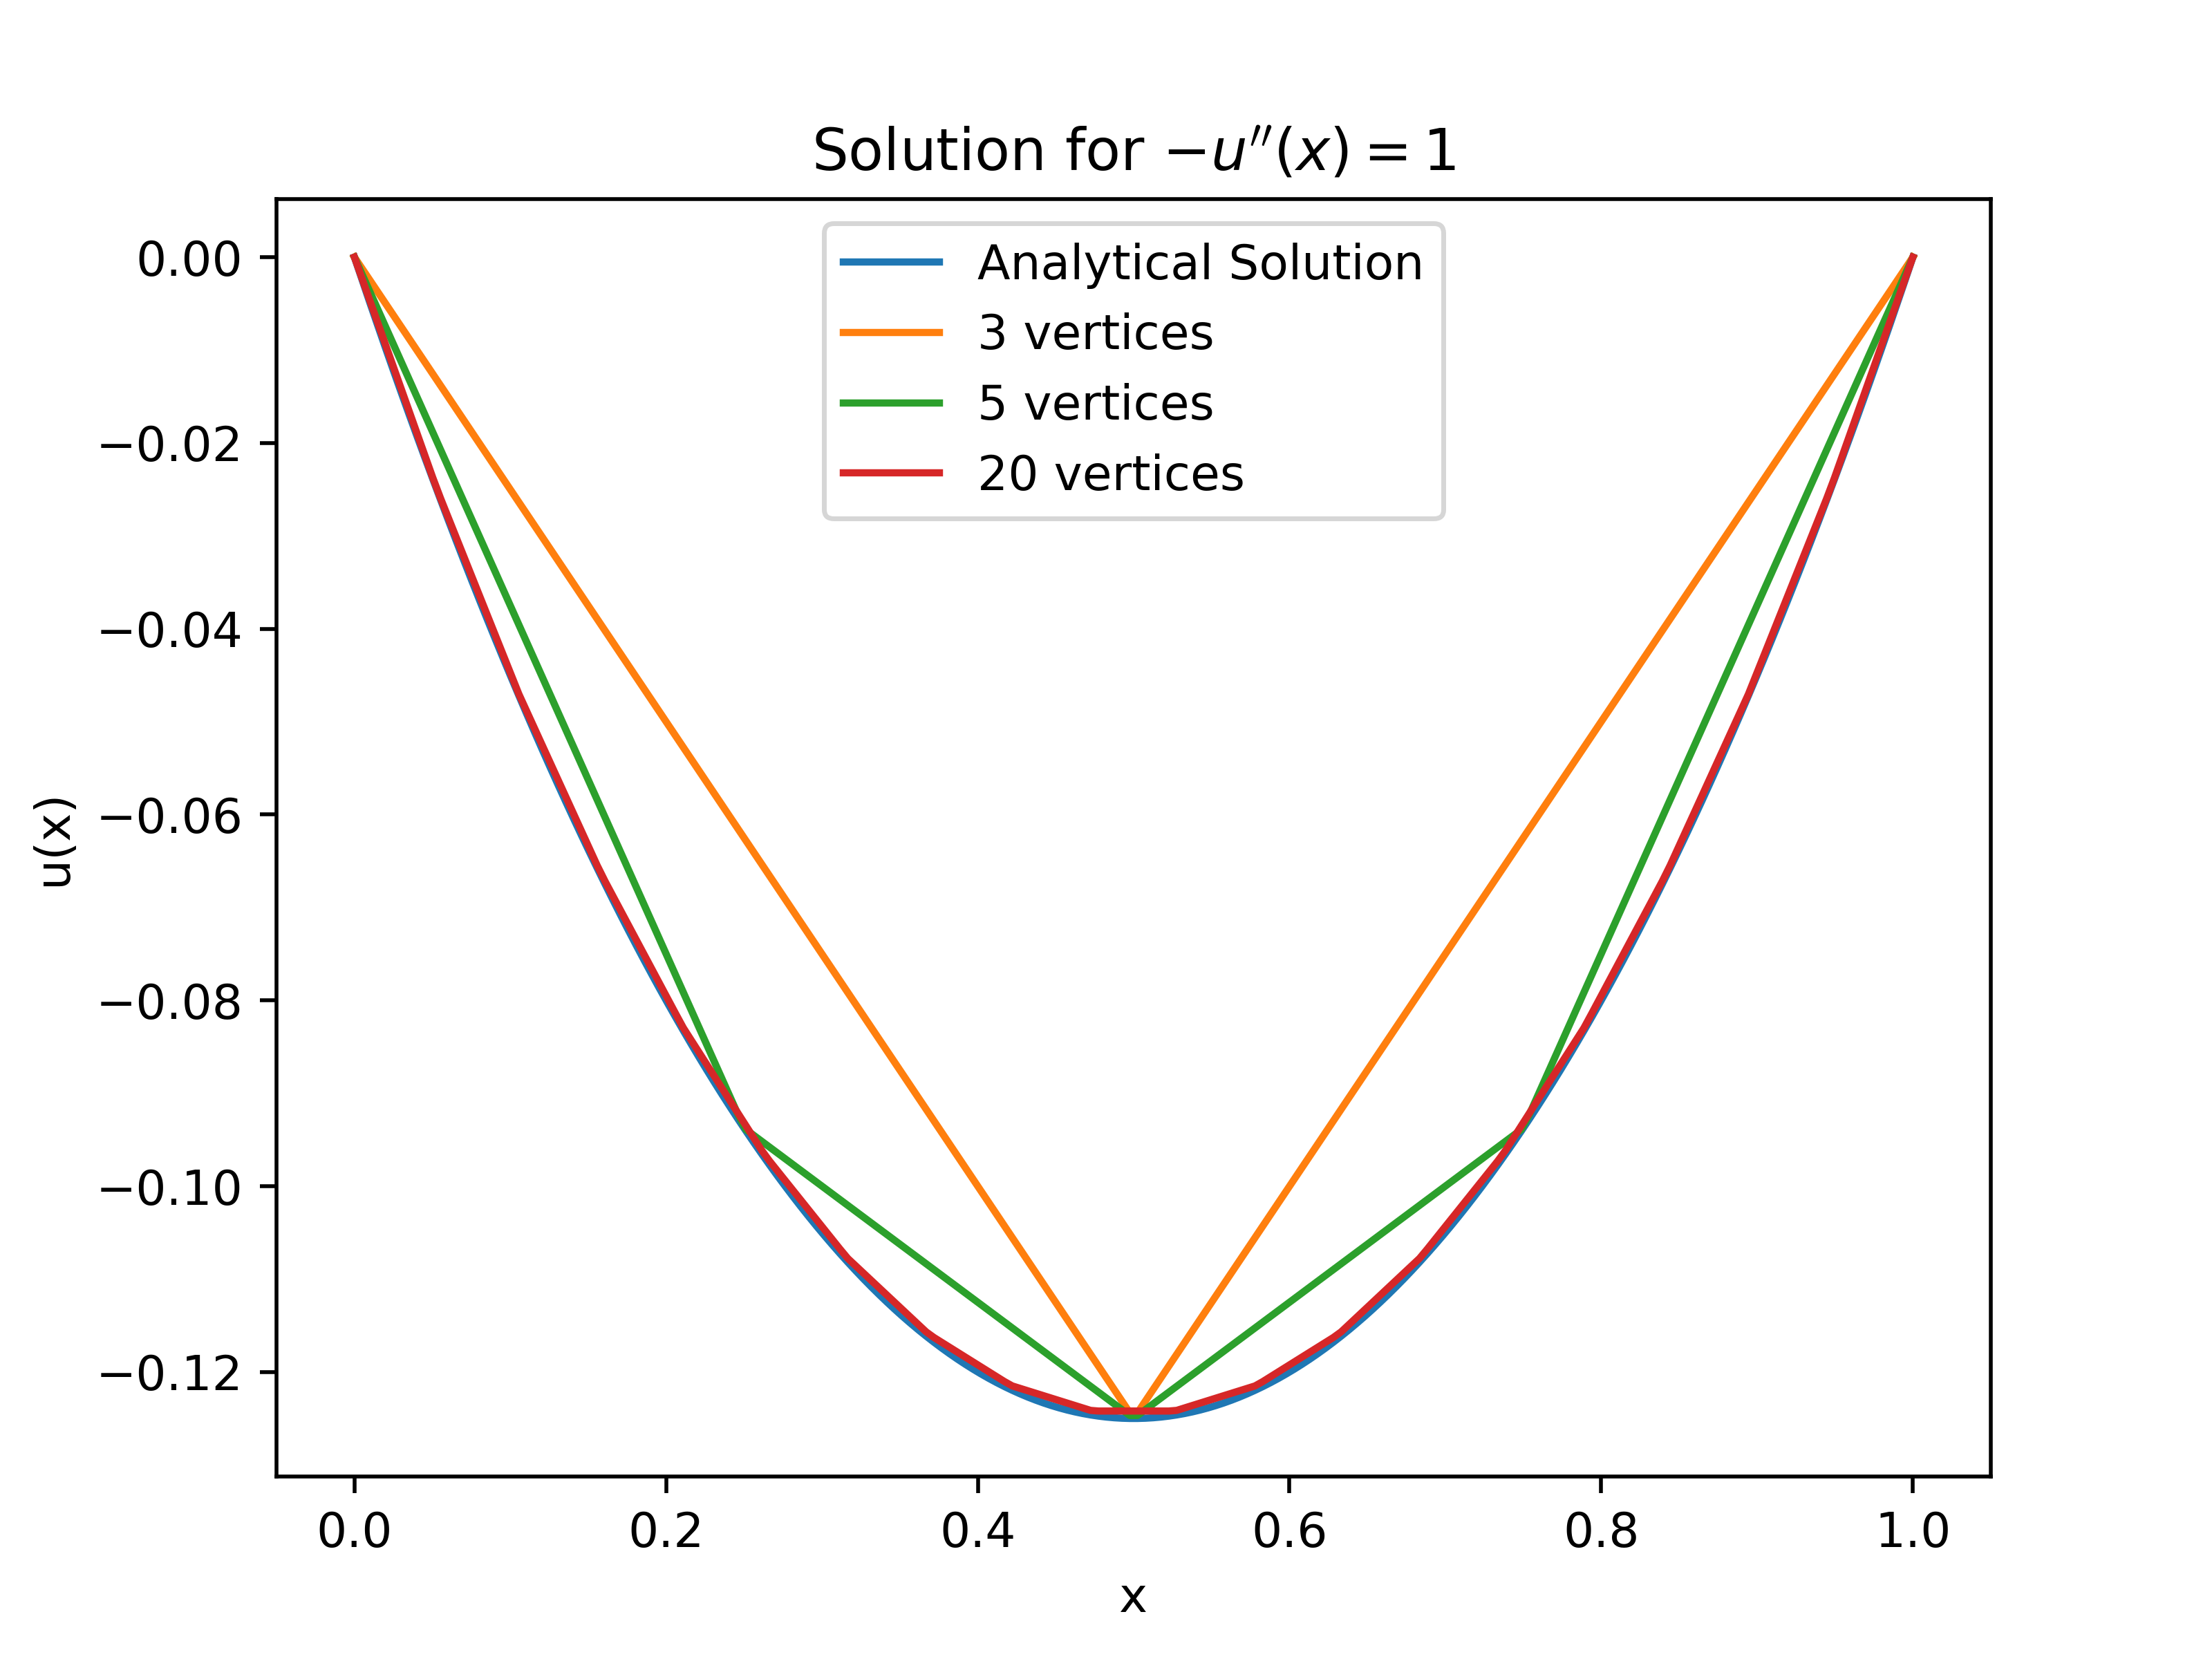
\includegraphics[width=8cm]{poisson 1d/(Poisson_1d)_(lin_sol).png}
    \caption{Solutions for various mesh sizes}
    \label{fig:Solution for given nodal points}

\end{minipage}%
\begin{minipage}{.5\textwidth}
    \centering
    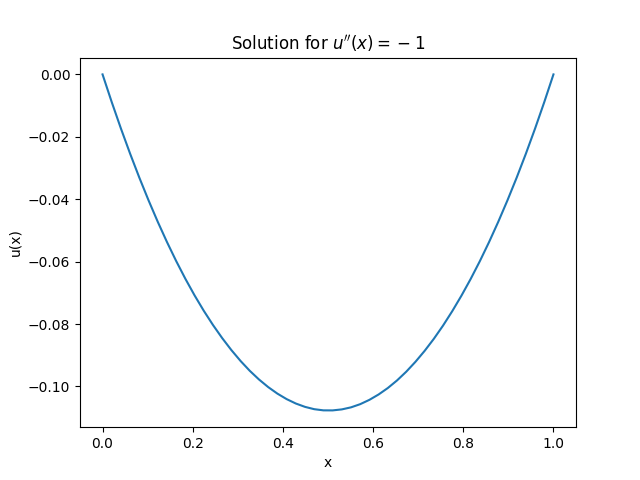
\includegraphics[width=8cm]{poisson 1d/(Poisson_1d)_(lin_sol)_(vertex_num_50).png}
    \caption{Solution for 50 nodal points}
    \label{fig:Solution for 50 nodal points}

\end{minipage}
\end{figure}
\\
\\
\\
If we choose $f = -x$, we obtain the following solution for $\vec{u}$:
\begin{figure}[hbt!]
    \centering
    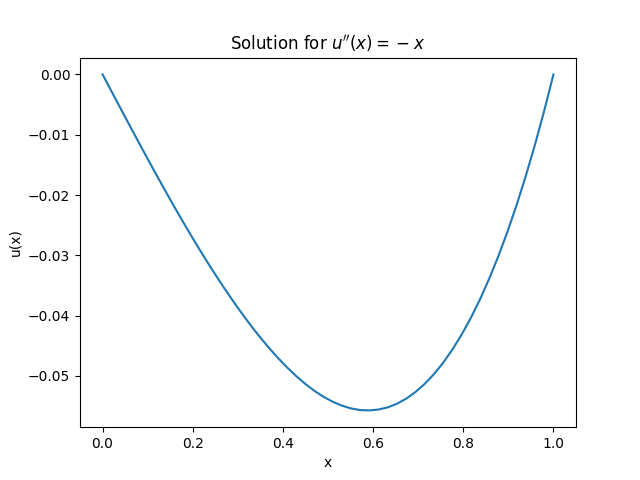
\includegraphics[width=10cm]{poisson 1d/(Poisson_1d)_(lin_sol)_(x)_(vertex_num_50).png}
    \caption{Solution for 50 nodal points}
    \label{fig:linear basis sum}
\end{figure}

\section{Two Dimensional Poisson Problem}
To solve the two dimensional Poisson problem, we wish to find a function $u(x,y)$ which satisfies 
\[-\nabla^{2}u = f\,\,\textrm{on }\Omega \quad \textrm{with Neumann and Dirichlet boundary conditions}.\]
Here the domain is a unit length square $[0,1]\times[0,1]$, and the Laplacian $\nabla^{2} =$ {\large$\frac{\partial^2}{\partial x^2}$} $+$ {\large$\frac{\partial^2}{\partial y^2}$}. The Neumann boundary conditions (boundary conditions on the directional derivative of $u$ as opposed to $u$ itself) are of the form $$\nabla u(x,y)\cdot \hat{n} = ?????x(x-1) \qquad \forall\, (x,y)\, \epsilon \,\partial\Omega,$$
and the Dirichlet boundary conditions are as before, $u(x,y) = 0 \, \textrm{on } \partial\Omega.$

The two dimensional Poisson problem can also be written in its weak formulation. We similarly multiply by a test function $\phi(x,y)$ on both sides of the equation, and integrate both sides over the entire domain. To do this, we must first define an infinite dimensional function space $V$ as follows:
$$V := \{v(x,y)| \,v, \nabla v \,\epsilon\, L^2(\Omega),  v = 0 \,\, \textrm{on } \partial\Omega\}.$$
Here $L^2(\Omega)$ is a space of functions which are square integrable on the given domain. The reason we need to introduce a slightly complicated function space, is to ensure uniqueness of a solution. When we proceed to search for solutions on our mesh, we could encounter problems of uniqueness of a function at the boundary of each cell. But since a line has Lebesgue Measure zero (meaning that a line in the real plane does not contribute to the value of an integral), we can surpass this problem by defining functions to be in a sense equal if they have the same "size", i.e. they are equal in their $L^2$ norm. 
Now we can find the weak formulation of the Poisson problem in the same way as we did previously. Multiplying by a test function a test function $\phi(x,y)$ on both sides of the equation, and integrating both sides over the entire domain.
\section{Non-Linear Poisson Problem}
\section{Heat Equation}
\section{References}
Understanding Navier-Stokes:
\begin{itemize}
\item https://doi.org/10.1590/1806-9126-RBEF-2017-0239
\item https://www.claymath.org/millennium/navier-stokes-equation/
\item 
\end{itemize}
Computational Methods:
\begin{itemize}
\item https://doi.org/10.1016/B978-1-4557-3141-1.50031-9
\item https://doi.org/10.1016/B978-0-12-824117-2.00011-9
\item https://doi.org/10.1016/B978-0-12-815601-8.50006-9
\end{itemize}
One Dimensional Poisson Problem:
\begin{itemize}
\item https://www.youtube.com/watch?v=P4lBRuY7pC4
\item https://jsdokken.com/dolfinx-tutorial/chapter1/fundamentals.html
\item Johnson, C. (n.d.). Numerical solution of partial differential equations by the finite element method. Courier Corporation.
\end{itemize}
Two Dimensional Poisson Problem:
\begin{itemize}
\item https://mathworld.wolfram.com/L2-Space.html
\end{itemize}
Non Linear Poisson Problem:
\begin{itemize}
\item 
\end{itemize}
Heat Equation:
\begin{itemize}
\item 
\end{itemize}

\end{document}
non linear Poisson Equation $-\nabla \cdot((u+1)\nabla u) = f$

While it was feasible to solve the aforementioned subproblems associated with the Navier-Stokes equations, combining our 